\subsection*{Packet Capturing}
\begin{frame}
\frametitle{Packet Capturing: Hardware View}
\begin{columns}
\column[t]{0.5\textwidth}
\vspace{-15em}
\begin{enumerate}
	\item \textbf{Receiving} network packets
		\begin{itemize}
			\item receive at network adapter
			\item DMA transfer in RAM \newline
		\end{itemize}
	\item \textbf{Filtering} the received packets 
		\begin{itemize}
			\item \emph{Berkeley Packet Filter}\newline
		\end{itemize}
	\item \textbf{Storing} to the hard disk
		\begin{itemize}
			\item using a system call
		\end{itemize}
\end{enumerate}
\column[t]{0.5\textwidth}
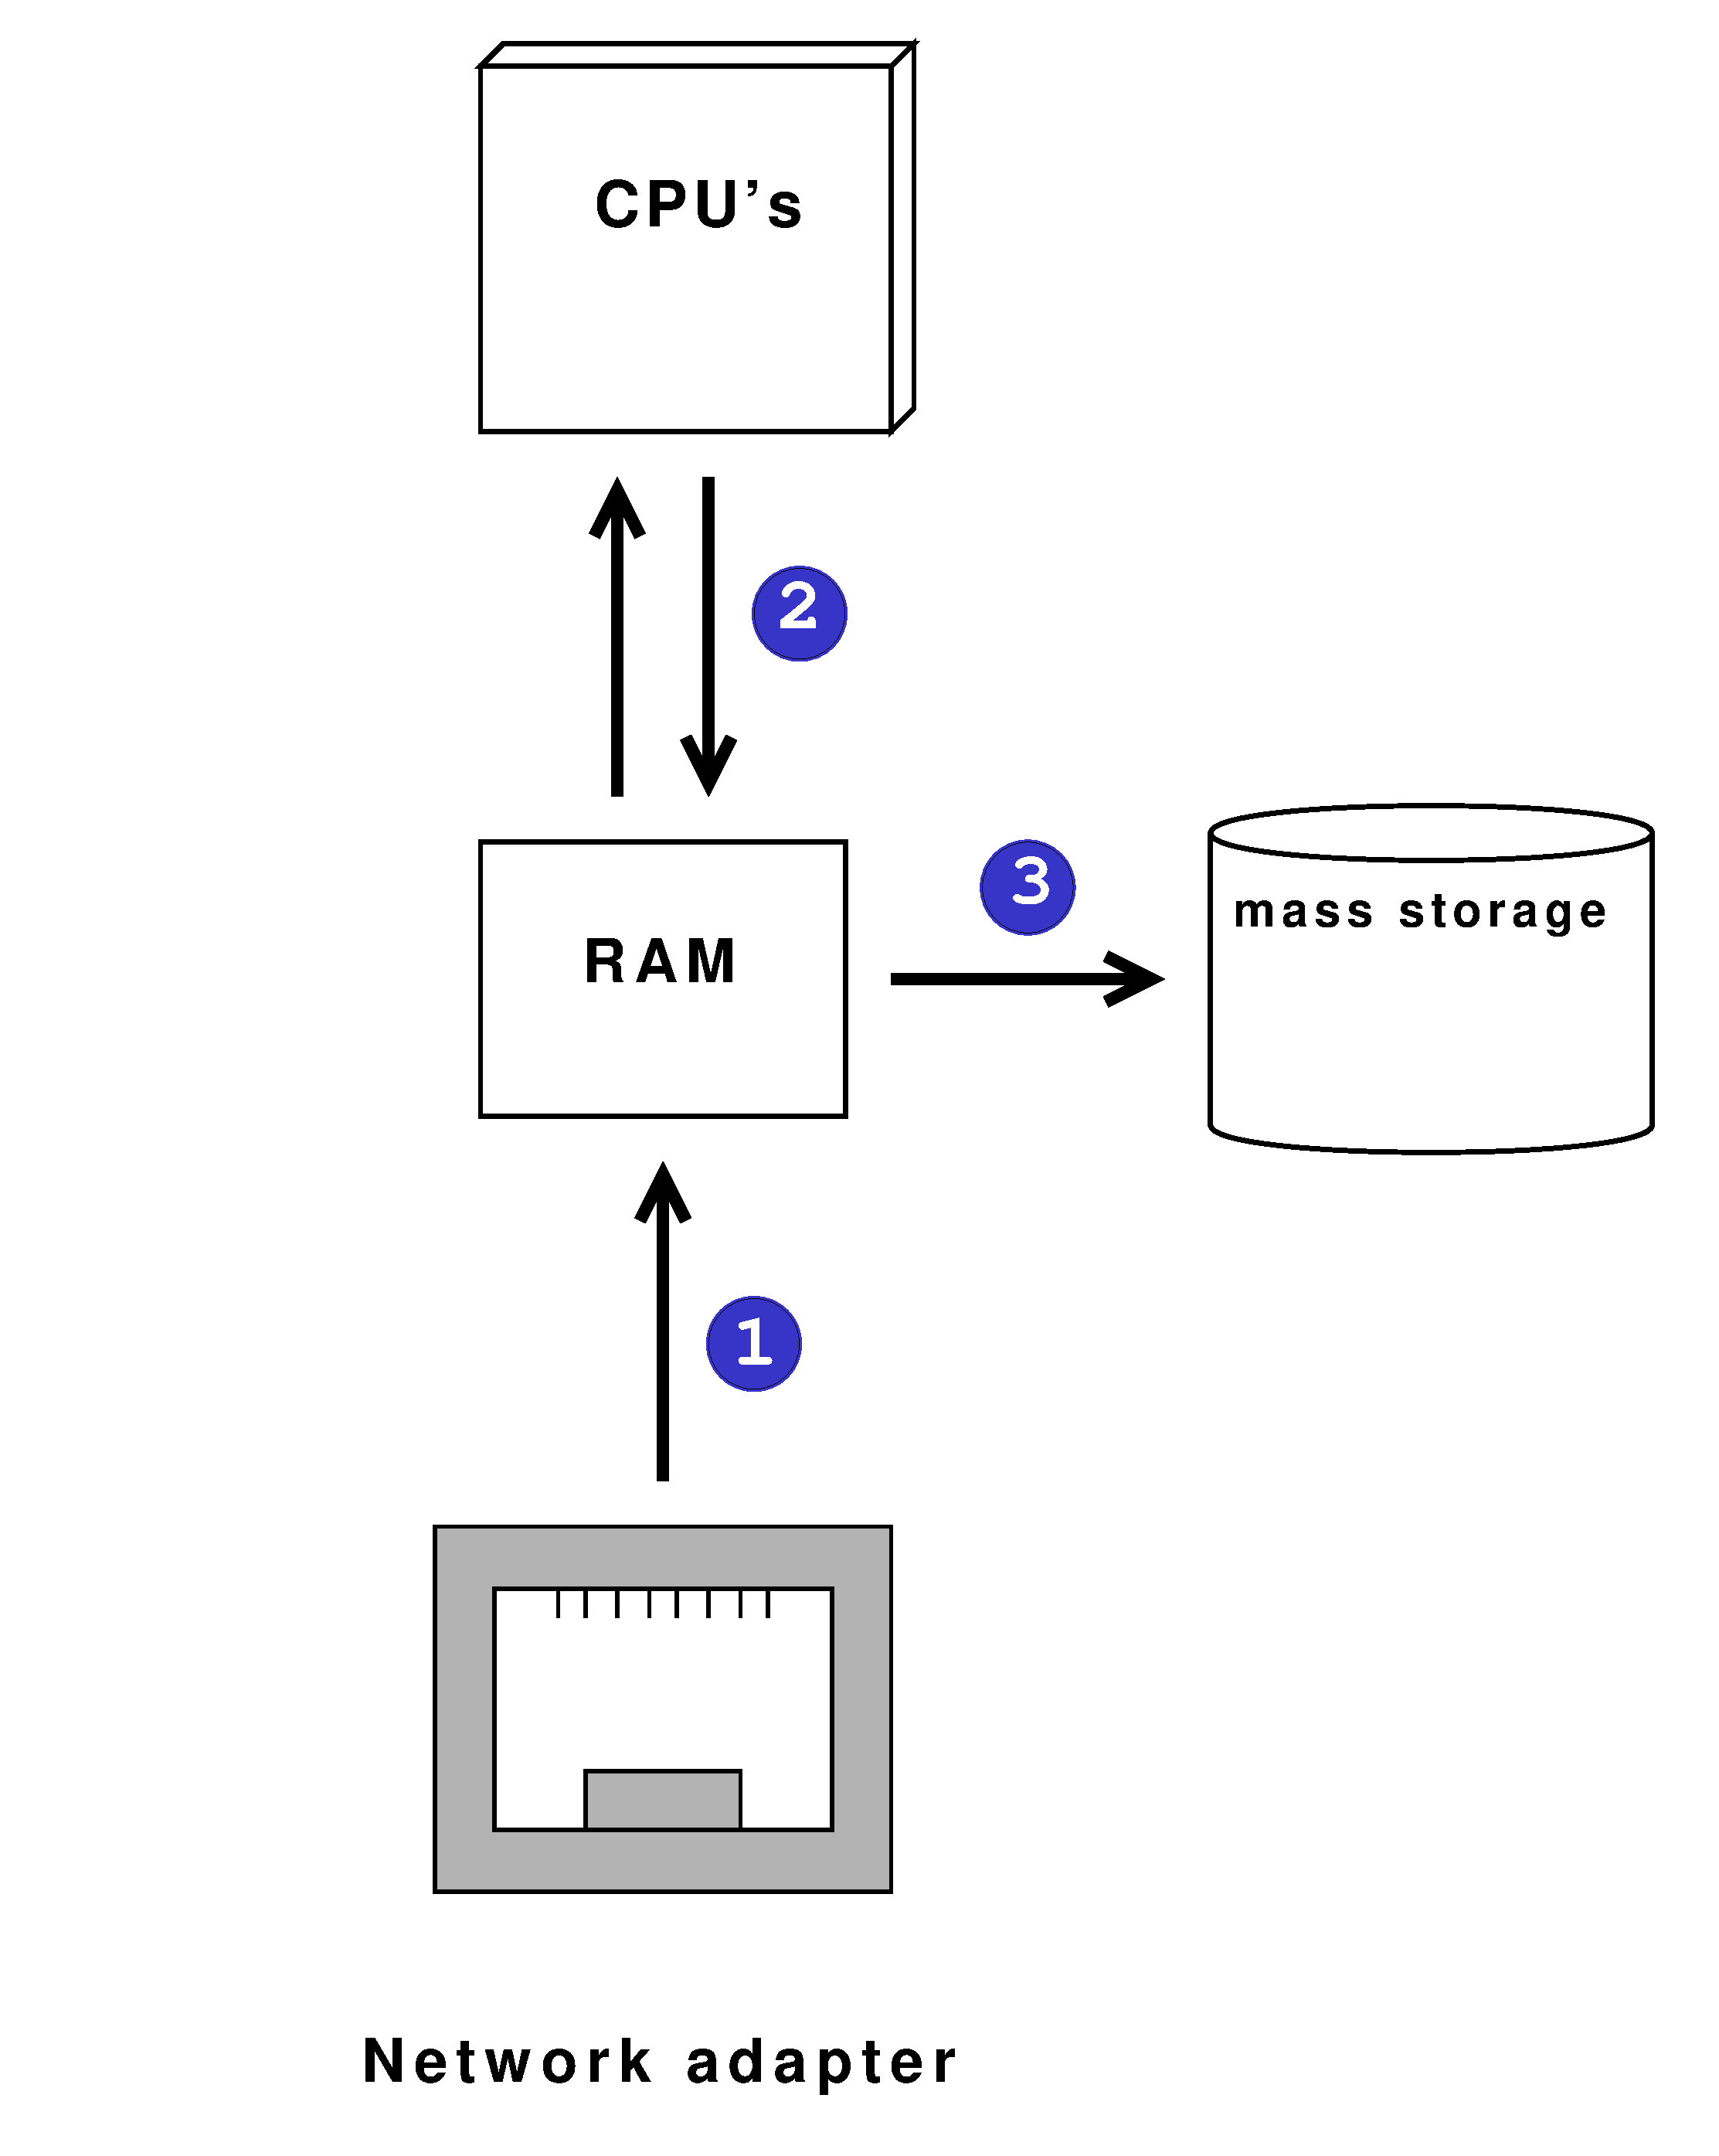
\includegraphics [width=0.82\textwidth, keepaspectratio]{pics/HardwareView}
\end{columns}
\end{frame}

\begin{frame}
\frametitle{FreeBSD Packet Capturing Stack}
\begin{itemize}
	\item \textbf{Network driver}
		\begin{itemize}
			\item Receiving packets\newline
		\end{itemize}
	\item \textbf{Berkley Packet Filter} (BPF)
		\begin{itemize}
			\item Filtering packets\newline
		\end{itemize}
	\item \textbf{User-space application}
		\begin{itemize}
			\item Accessing received packets
			\item Initiates:
				\begin{itemize}
					\item Storing packets to hard drive
					\item Output packets information to the terminal
				\end{itemize}
		\end{itemize}
\end{itemize}
\end{frame}

\subsection*{How does it work}
\begin{frame}
	\begin{center}
	\huge{How does standard packet capturing work}
	\end{center}
\end{frame}

\begin{frame}
\frametitle{FreeBSD Standard Packet Capturing Stack}
\begin{columns}
\column[t]{0.5\textwidth}
\vspace{0em}
\newline
\begin{itemize}
\item <6-> Access packets
\item <5-> Packet filtering
\item <4-> Interrupt Service Routine
\item <3-> Interrupt
\item <2-> DMA-Transfer
\item <1-> Packet is received and saved in Adapter-FIFO
\end{itemize}
\column[t]{0.5\textwidth}
\vspace{-2em}
\begin{figure}
	\only<1>{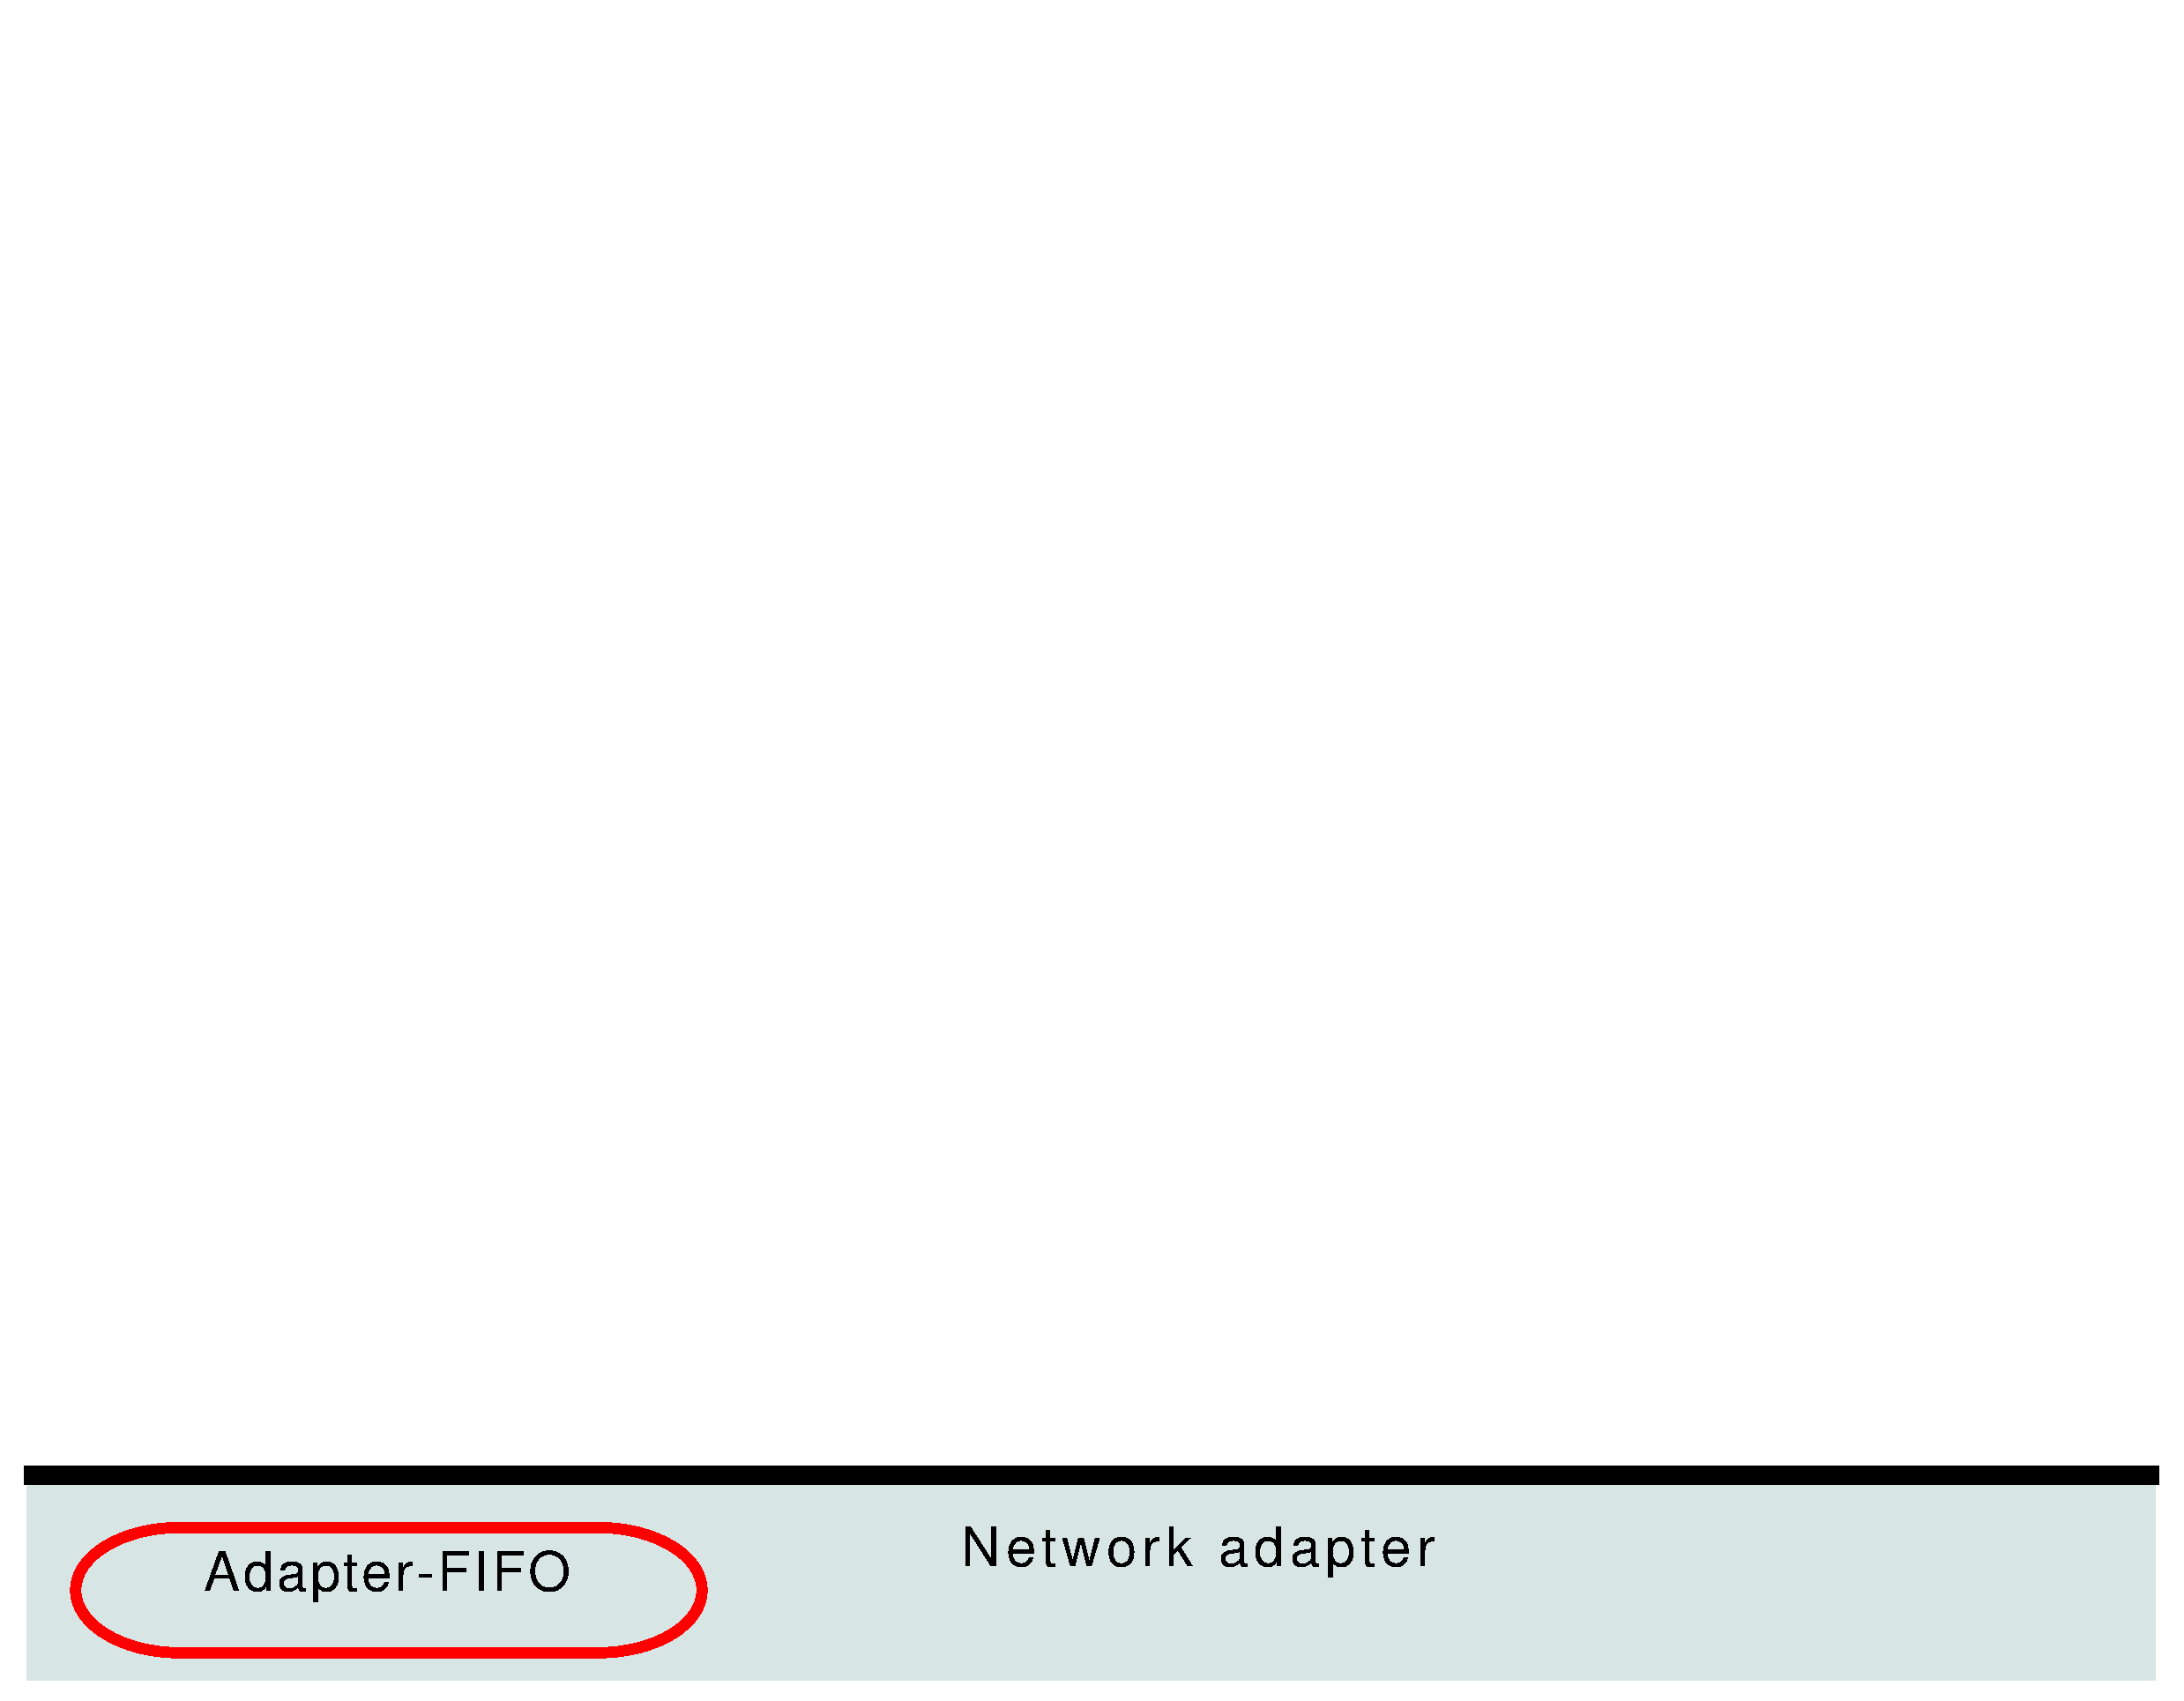
\includegraphics [height=55mm,width=60mm]{pics/3copy_0}}
	\only<2>{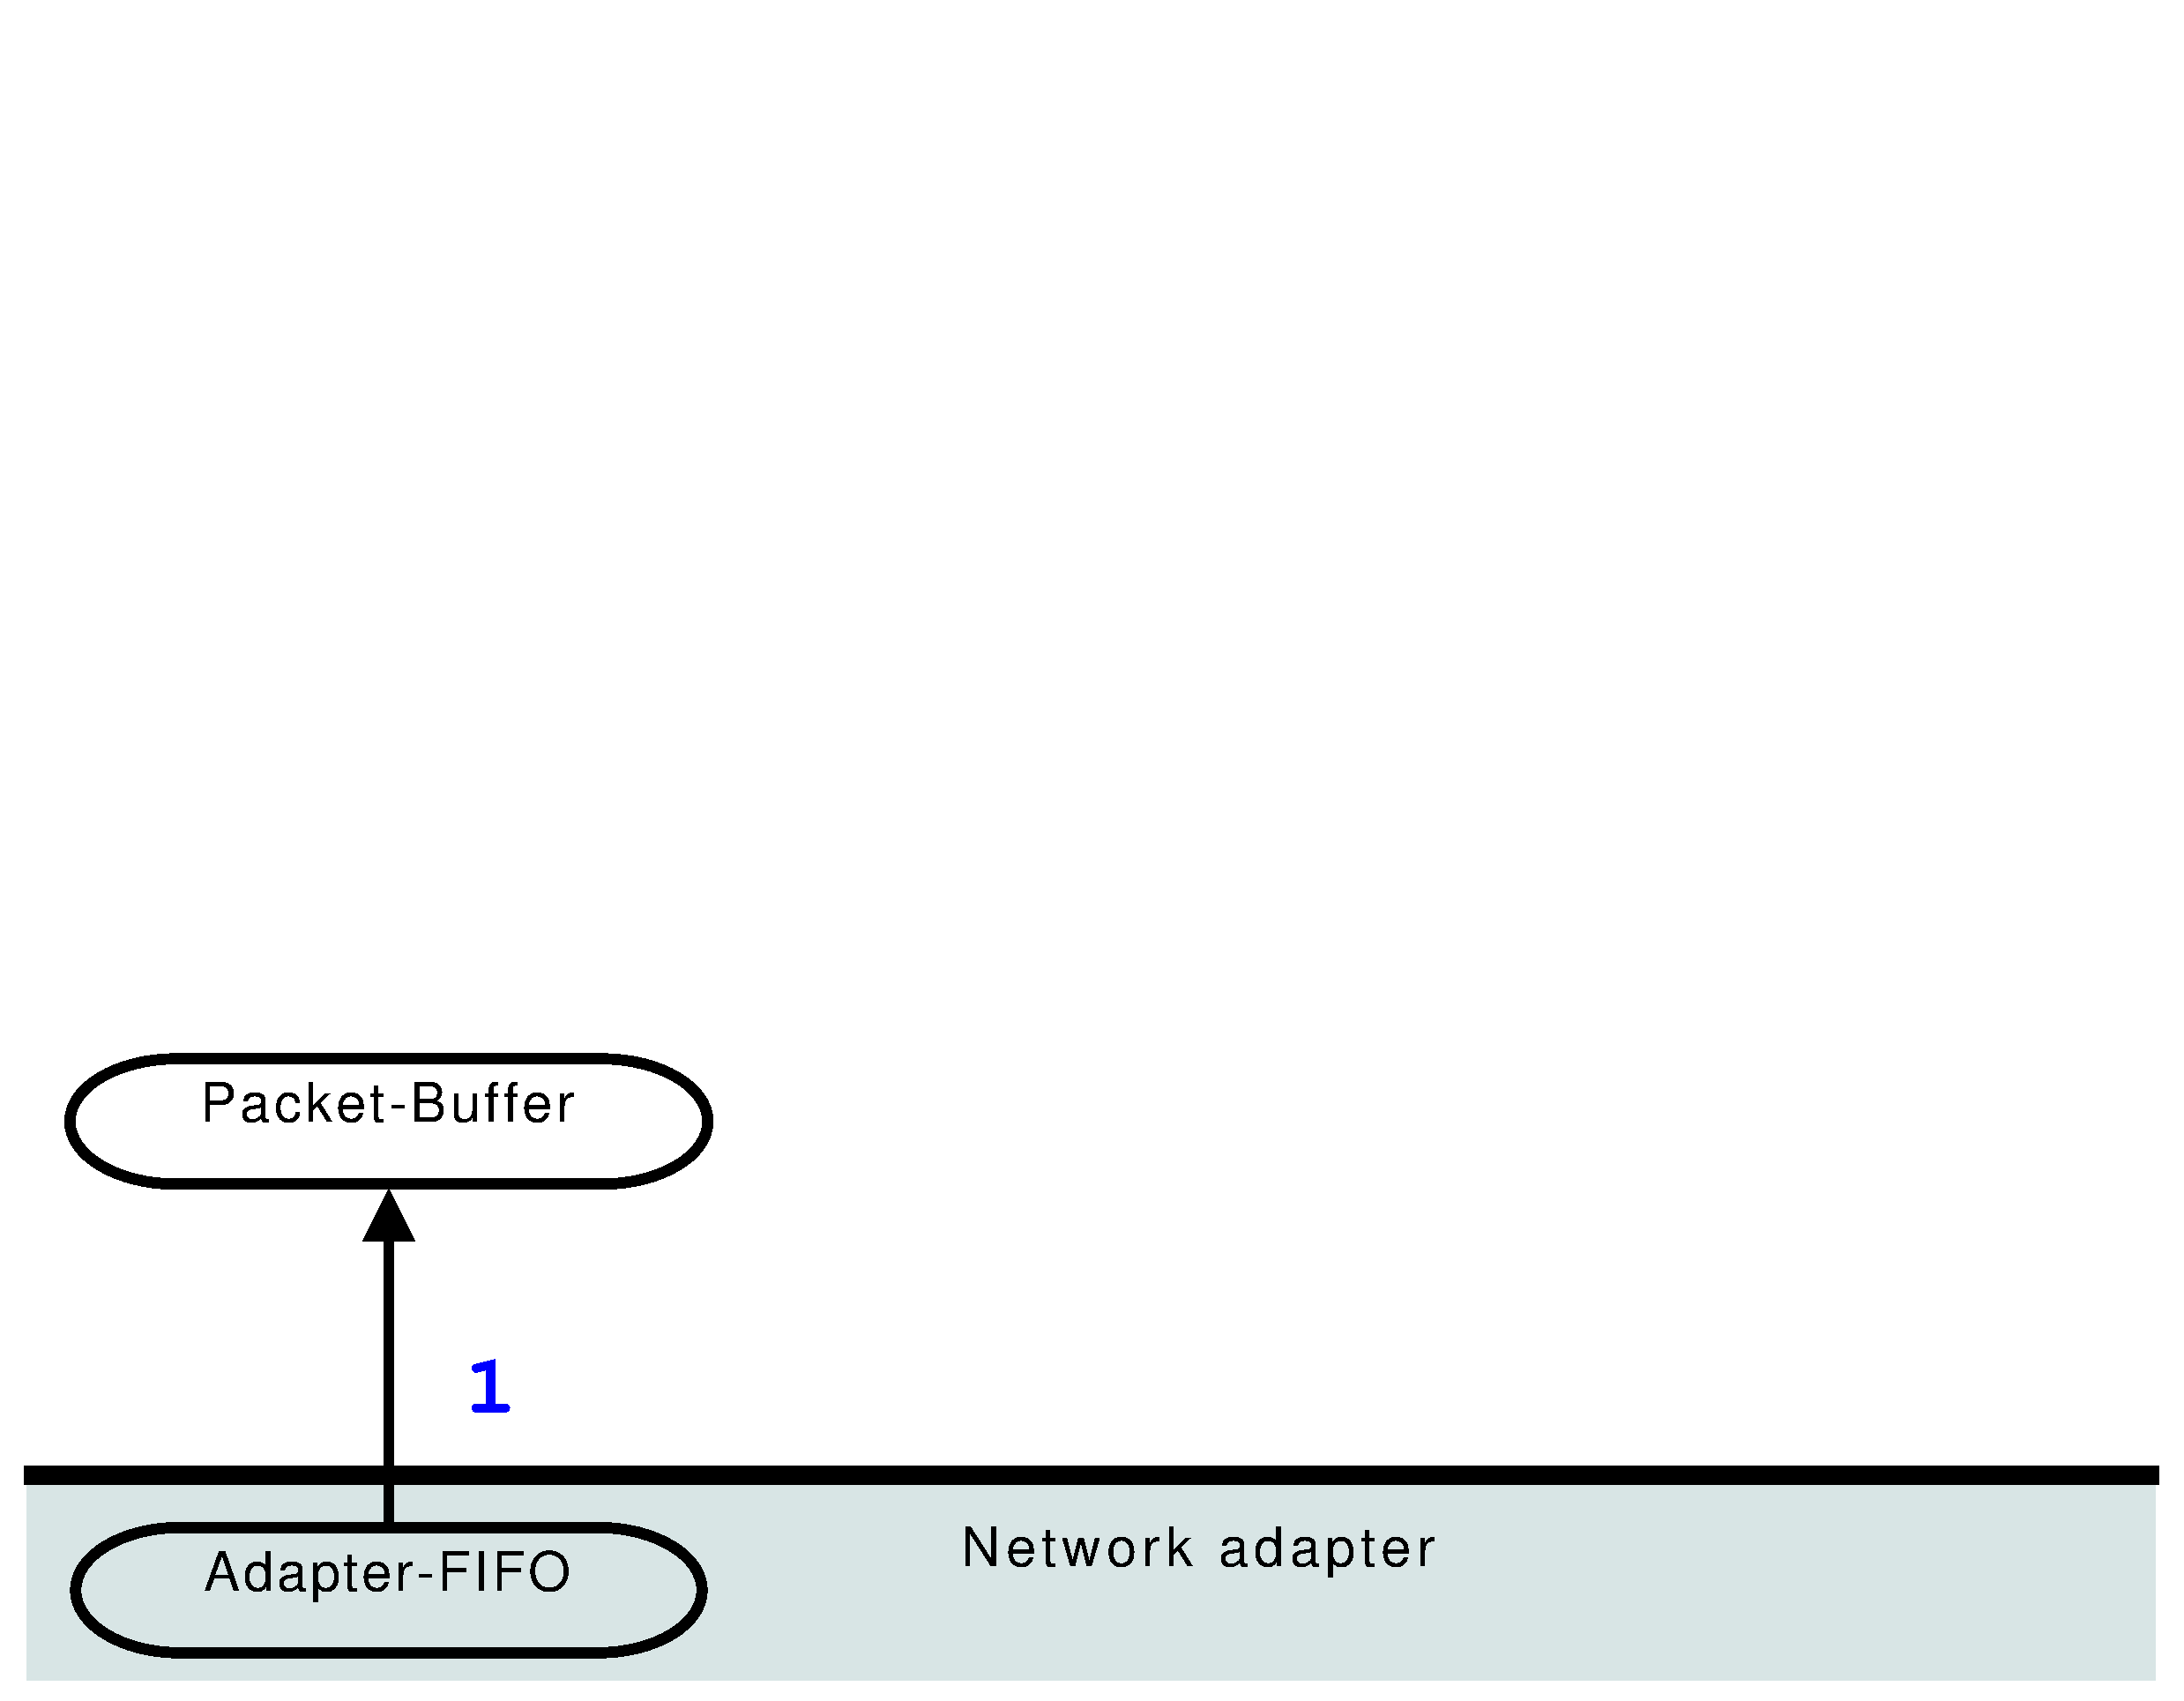
\includegraphics [height=55mm,width=60mm]{pics/3copy_0.5.eps}}
	\only<3>{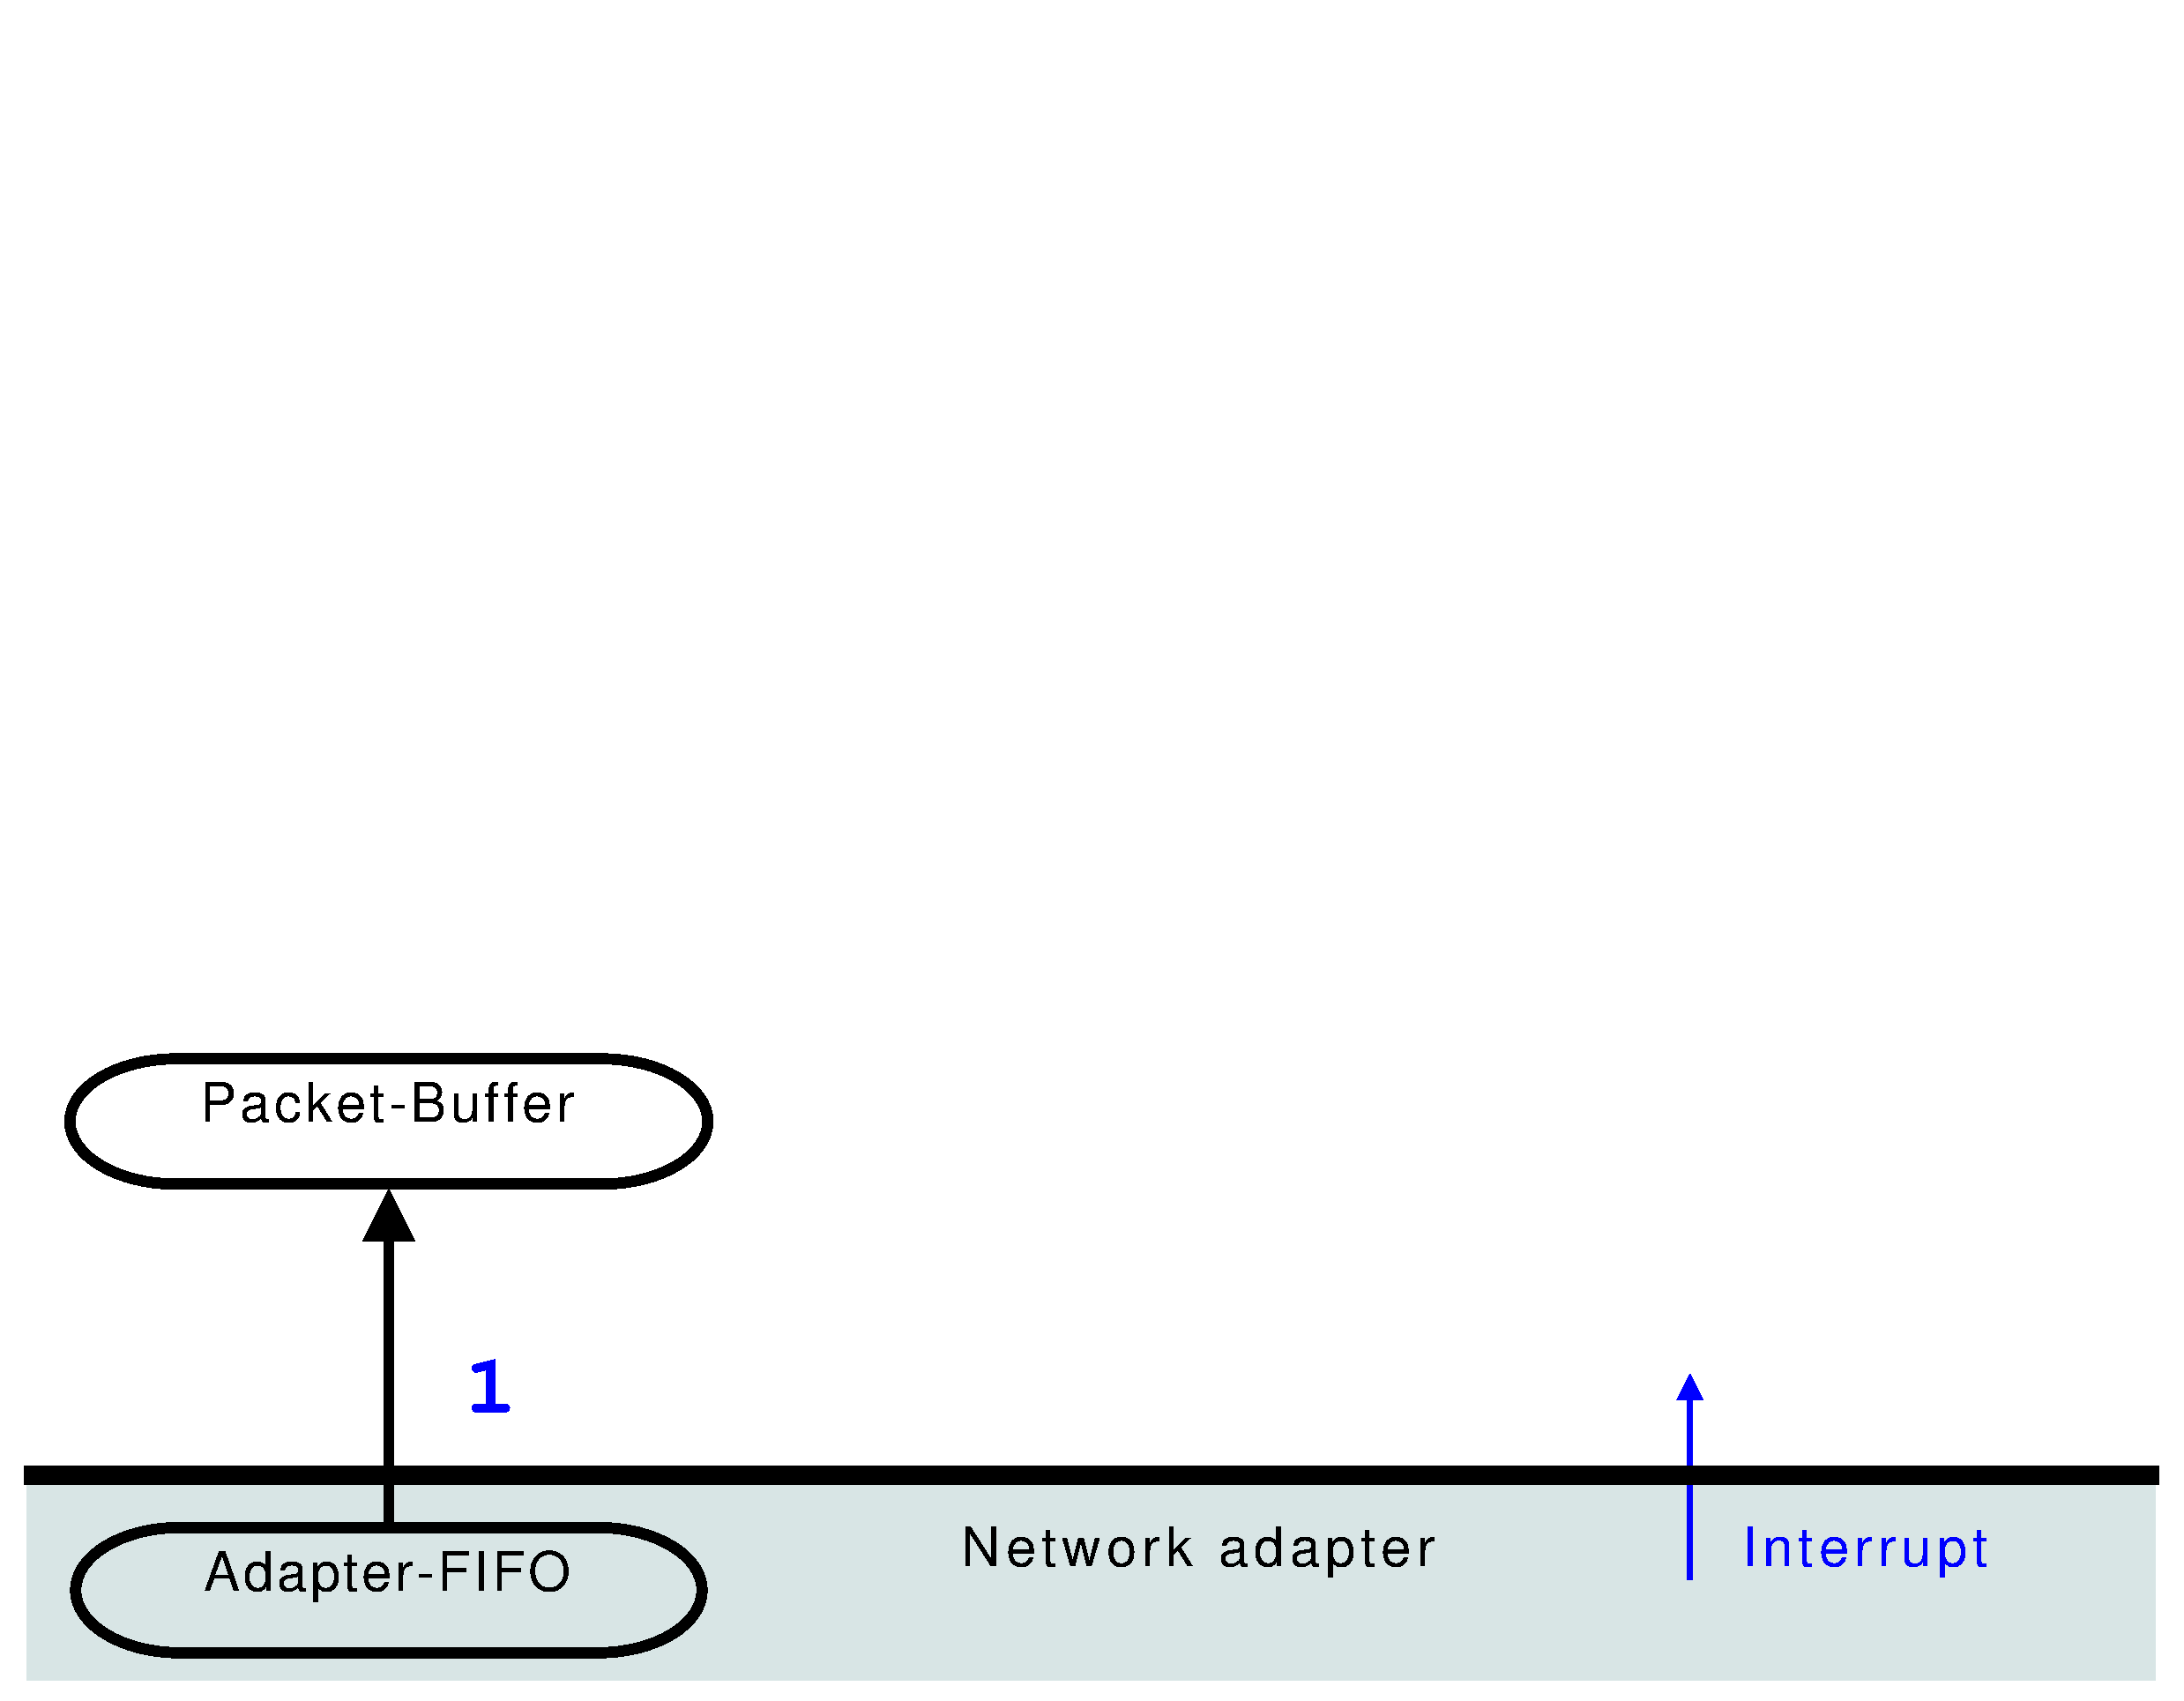
\includegraphics [height=55mm,width=60mm]{pics/3copy_0.7.eps}}
	\only<4>{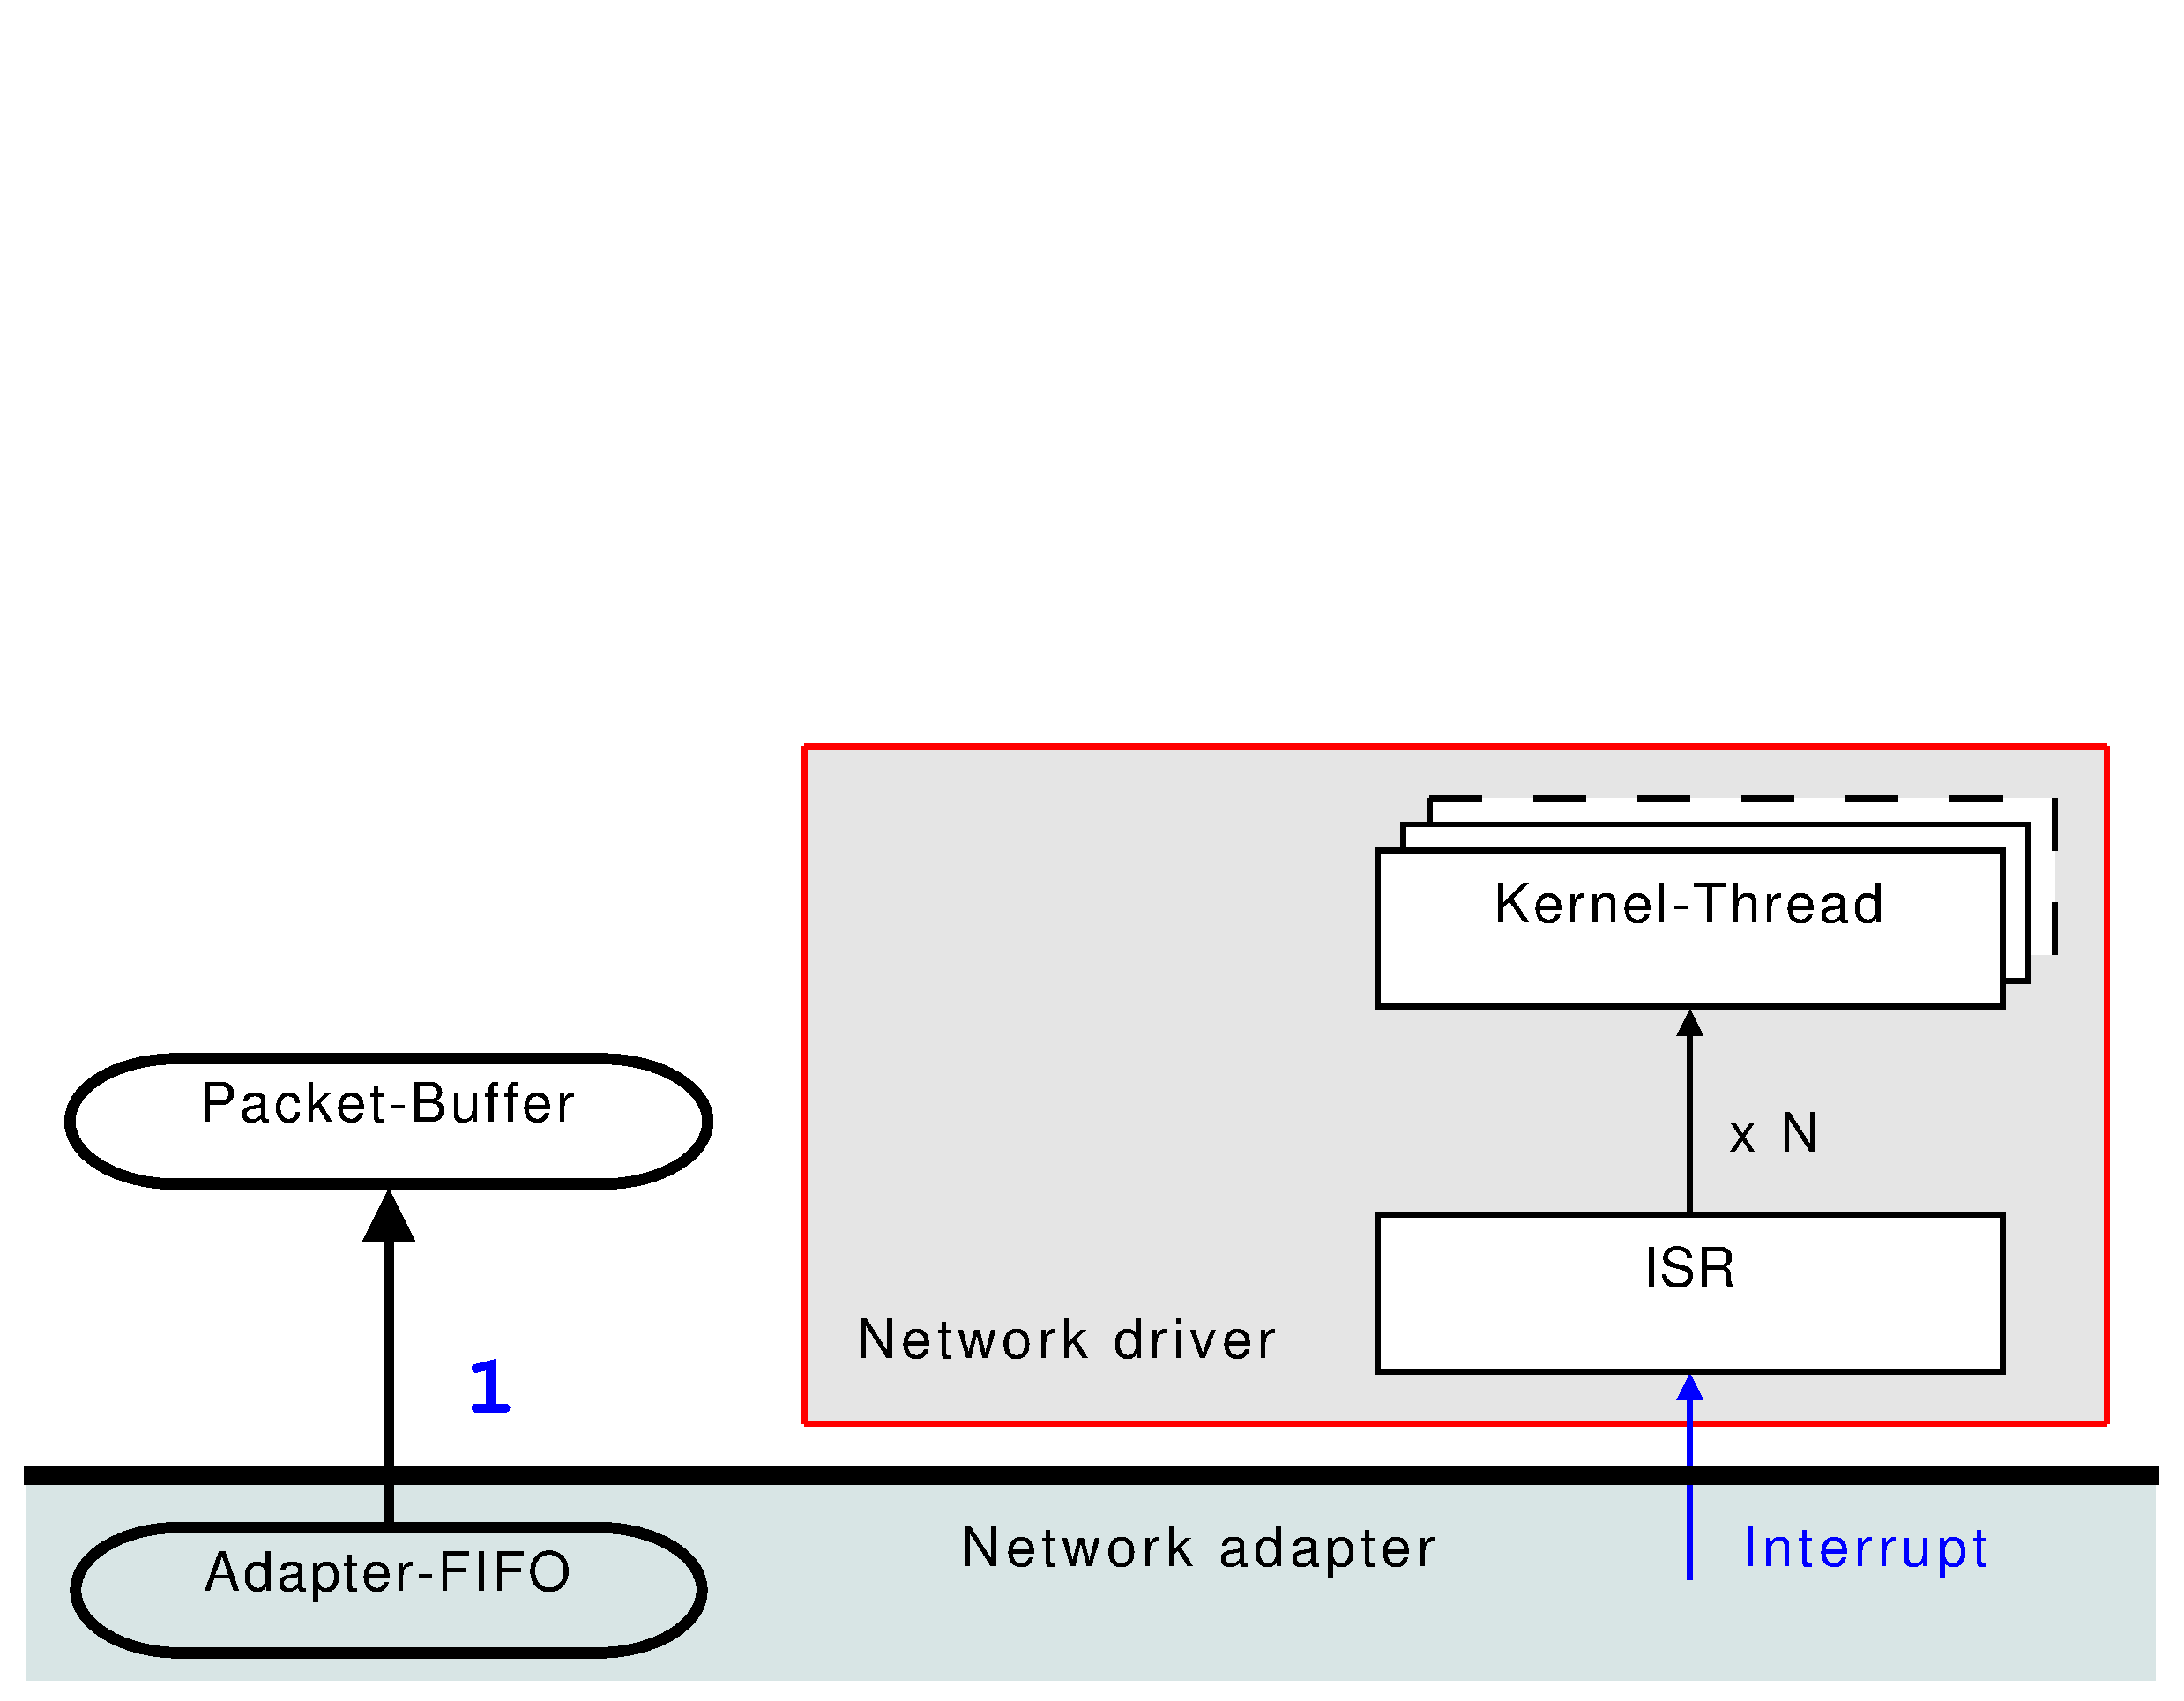
\includegraphics [height=55mm,width=60mm]{pics/3copy_1}}
	\only<5>{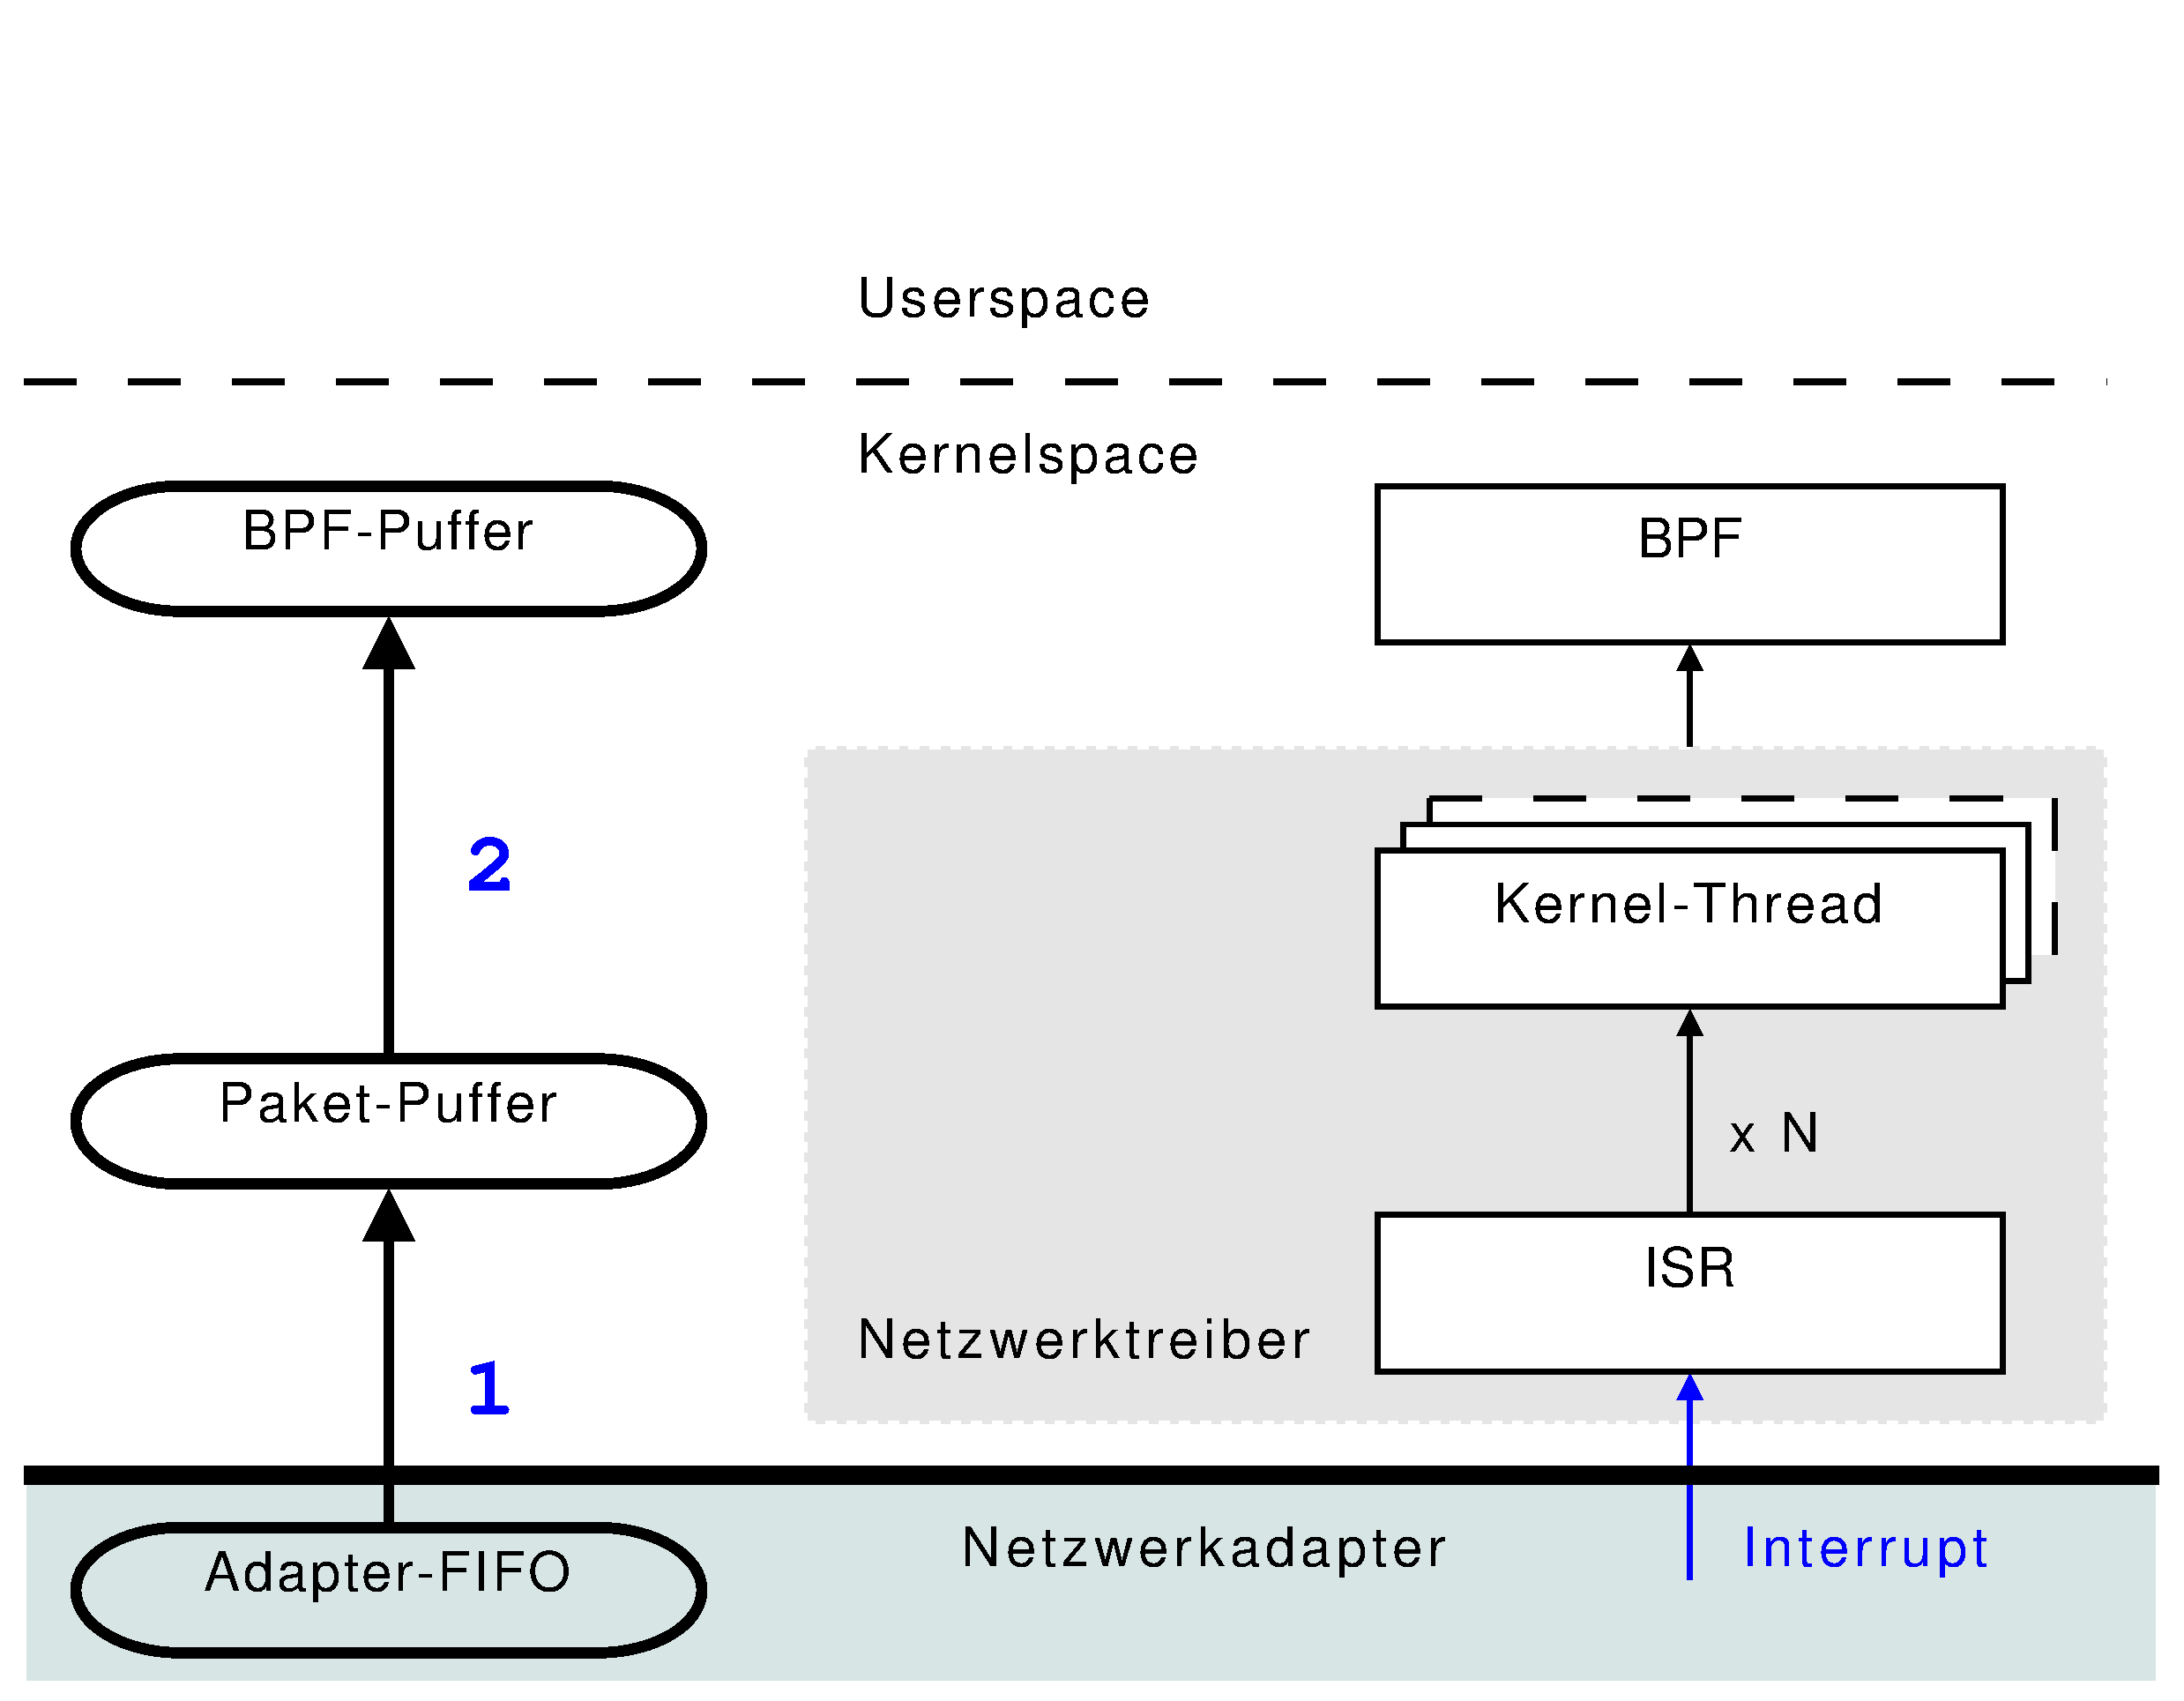
\includegraphics [height=55mm,width=60mm]{pics/3copy_2}}
	\only<6>{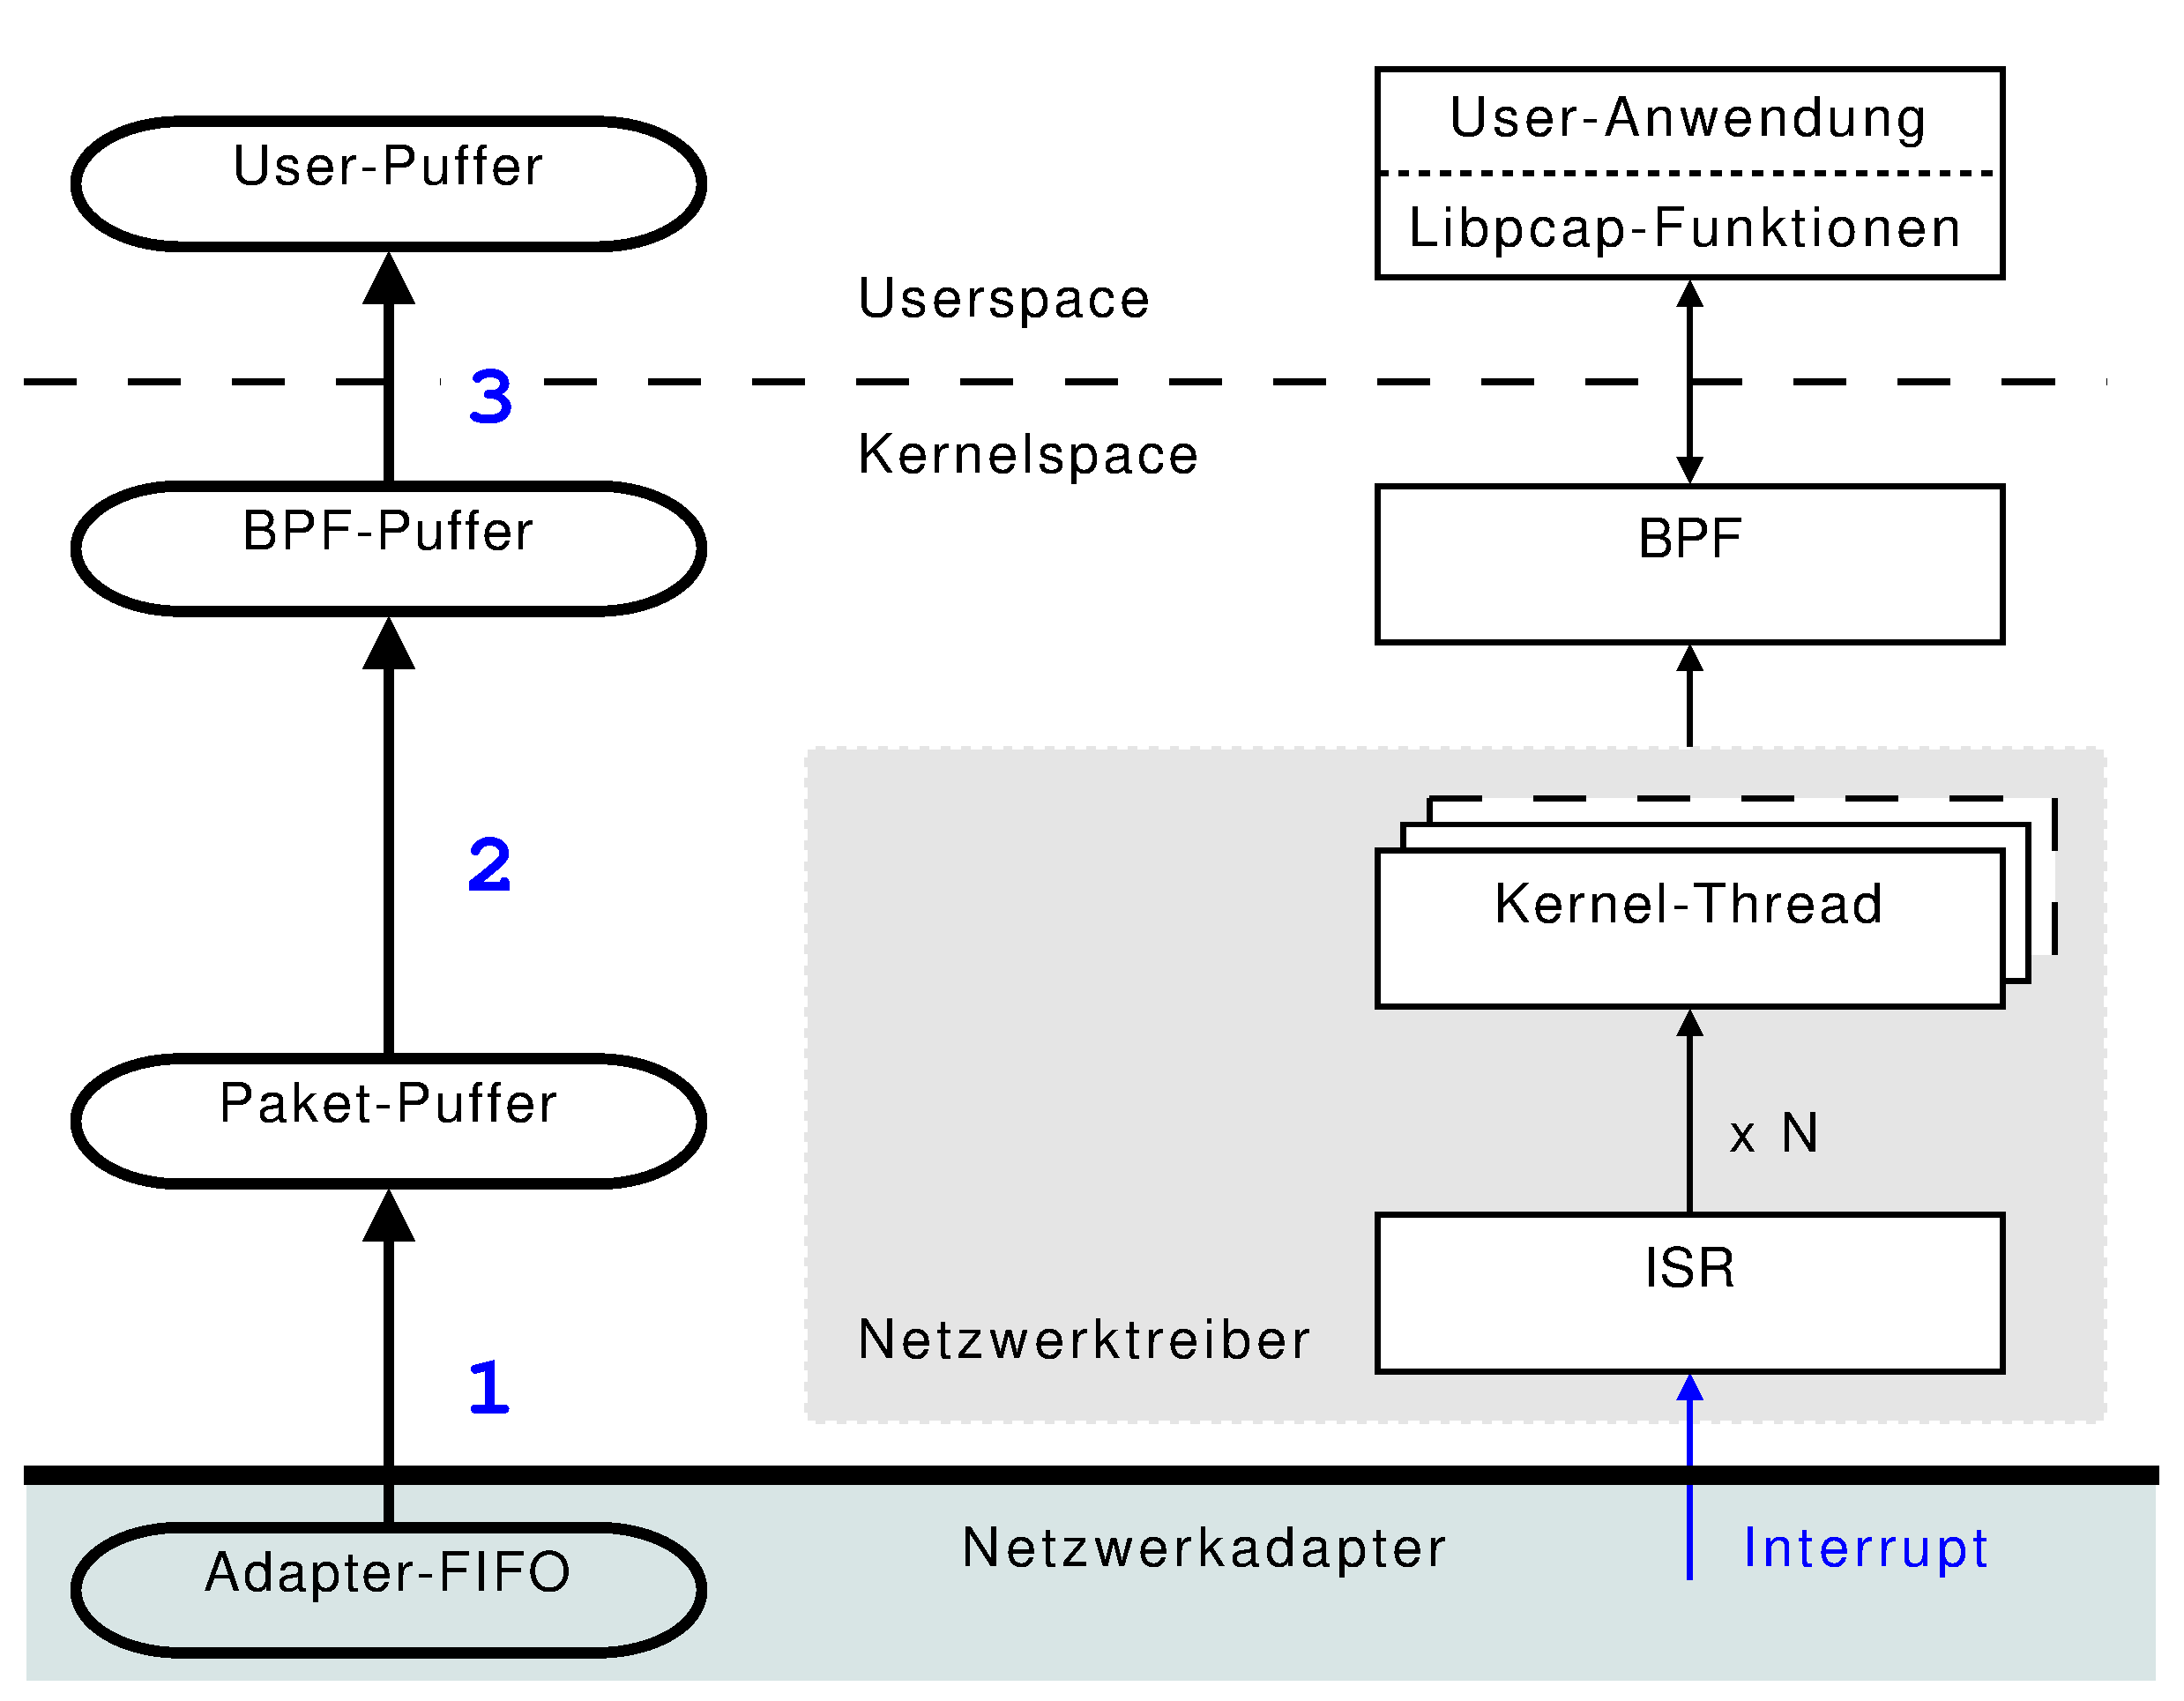
\includegraphics [height=55mm,width=60mm]{pics/3copy_3}}
\end{figure}
\end{columns}
\end{frame}


\subsection*{Disadvantages of standard capturing software}
\begin{frame}
\frametitle{Disadvantages of Standard Packet Capturing Stack}
\begin{itemize}
	\item<1-> Memory allocations
		\begin{itemize}
			\item<1-> For each new received packet a new \emph{mbuf} 
				is allocated\newline
		\end{itemize}


	\item<2-> Too many packet copies
		\begin{itemize}
\ifthenelse{\boolean{SUMMIT}}{
			\item<2-> DMA: $Controller \Rightarrow RAM$
			\item<2-> BPF: $RAM \Rightarrow RAM (BPF\ Buffer)$
			\item<2-> read(2): $RAM \Rightarrow RAM (Userspace\ Buffer)$\emph{(*)}\newline
}{
			\item<2-> DMA: $FIFO \Rightarrow Packet\ Buffer$
			\item<2-> $Packet\ Buffer \Rightarrow BPF\ Buffer$
			\item<2-> $BPF\ Buffer \Rightarrow Userspace\ Buffer$\emph{(*)}\newline
}
		\end{itemize}

	\item<3-> System calls
		\begin{itemize}
			\item<3-> User-space application receives the packets using read(2)\emph{(*)}
			\item<3-> Saving packets to the hard disk\newline
		\end{itemize}

\end{itemize}
\begin{tiny}
\emph{(*)} Using Zero-Copy BPF eliminates the last copy and system call
\end{tiny}
\end{frame}

